\section{Results}
\subsection{Calibration}
Defects in the geometry of the antenna can lead to the maximum of the sensitivity to not be properly aligned with the pointing of the antenna.
It is necessary to calibrate in order to be able to apply the correction for later measures.


The sun is the strongest discrete radio source in the sky\cite{burke_introduction_2013}. \hl{Details d'où vient le signal etc}.
The first preliminary measures indicated a maximum of the signal power a point to the bottom left of the sun.
Therefore a series of measures were made in order to draw a grid to the bottom left of the sun. The position of the sun was recorded for each measure in order to study the relative position.
By interpolating the obtained values of power, the contour map depicted in \autoref{fig:calibration_contour} was obtained.
One can see how the maximum is at Az/Alt $\sim -5^{\circ}, -3^{\circ}$ of the actual position of the sun.

[aussi \cite{lauterbach_radio_2022} parle du soleil, section 4.1]

\begin{figure}[htbp]
    \centering
    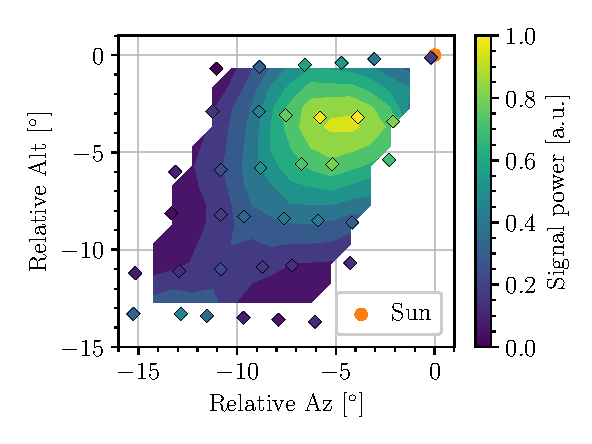
\includegraphics[scale=1]{figures/calibration_contour.pdf}
    \caption{Calibration contour}
    \label{fig:calibration_contour}
\end{figure}

\subsection{Distinguishing signal and noise}
Measure BM building, measure actual H21 source, divide actual by noise to extract the signal from noise, apply some filter and voilà, a nice signal

\subsection{Velocity field of the Milky Way}
Probing arms of milky way

Talk about orientation (i.e. sky visible at measuring time), correct angular momentum?
